\chapter{Literature Review}% Main chapter title
\thispagestyle{nohead}
\label{LitReview} % For referencing the chapter elsewhere, use \ref{LitReview} 

%----------------------------------------------------------------------------------------

This chapter views \where~as incorporating ideas from three separate disciplines: software verification, machine learning, and software measurement and metrics. 
%Each of these disciplines has a considerable body of research associated with it.
A Venn diagram illustrating the intersections of these disciplines and how this chapter is organised according to these intersections is given in Fig. \ref{fig:litreview}. 
We shall concentrate this review on Software Verification and SV research incorporating concepts from the other two disciplines. 
Where more background in associated topics outside the SV domain is required, the literature is discussed in the relevant sections (i.e. Sec. \ref{sec:lrmm} and \ref{sec:lrml}).

The rest of this chapter will review the literature associated with each segment of Figure \ref{fig:litreview} -- moving clockwise from the top. 
This review was approached with the following questions:
\begin{itemize}
	\item[\textbf{Q1}] What does the SV tool landscape look like in terms of interoperability?
	\item[\textbf{Q2}] Does a standardised suite of benchmark programs exist for the comparison of deductive SV tools?
	\item[\textbf{Q3}] How have concepts from traditional SE been applied to large-scale SV projects?
	\item[\textbf{Q4}] How have machine learning concepts been integrated for use in the SV domain?
\end{itemize}
The answers to these questions have informed the design choices made in regard to the \where~portfolio-solving tool.

\begin{figure}

\centering
\def\firstcircle{(3cm,0cm) circle (2.5cm)}
\def\secondcircle{(0cm,0cm) circle (2.5cm)}
\def\thirdcircle{(1.5cm,3cm) circle (2.5cm)}
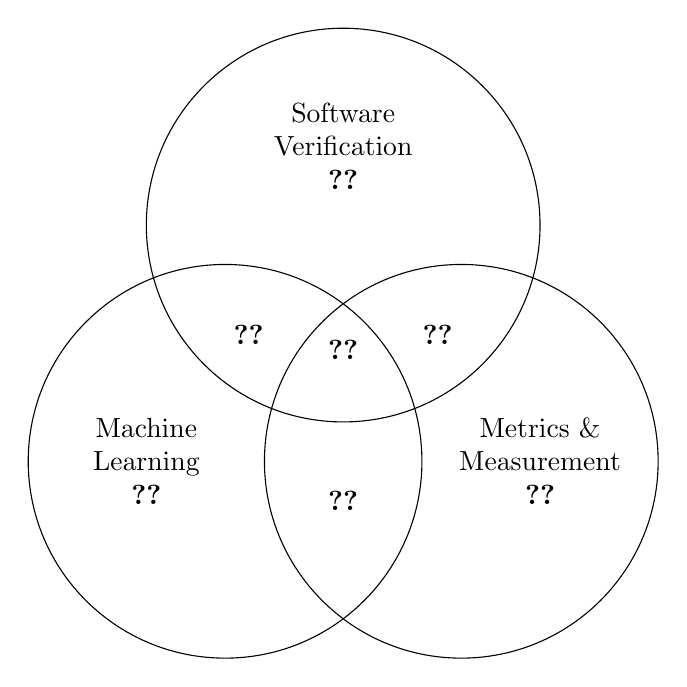
\begin{tikzpicture}
	
	\draw \firstcircle node [below] {};
	\draw \secondcircle node [above] {};
	\draw \thirdcircle node [below] {};
	\node[align=center] at (-1cm, 0cm) {Machine\\Learning\\ \ref{sec:lrml} };
	\node[align=center] at (1.5cm, 4cm) {Software\\Verification\\ \ref{sec:lrsv}};
	\node[align=center] at (4cm, 0cm) {Metrics \&\\ Measurement\\ \ref{sec:lrmm}};
	\node[align=center] at (1.5cm, 1.2cm) {\ref{sub:lrsvmmml}\\\small{\where} };
	\node[align=center] at (0.3cm, 1.6cm) {\ref{sub:lrsvml}};
	\node[align=center] at (2.7cm, 1.6cm) {\ref{sub:lrsvmm}};
	\node[align=center] at (1.5cm, -0.5cm) {\ref{sub:lrmmml}};
	
\end{tikzpicture}

\caption{\where~is placed at the intersection of three disciplines}
\label{fig:litreview}

\end{figure}


\section{\textsf{Why3} and Software Verification Systems}
\label{sec:lrsv}

\sloppypar
An overview of the \textsf{Why3} verification system \cite{why:shephard,why:whereprovers} has been given in the previous chapter. The WhyML programming language provides a high-level \texttt{ML}-like language for the specification of programs with pre- and post- conditions, recursive definitions and type invariants. An extensive library of verified polymorphic data-types make WhyML a flexible language \cite{verifythis,why:polymorphic}. 
It is \textsf{Why3}'s driver-based approach to interfacing with external tools that is of most interest to our project. 
The \textsf{Why3} approach is, in this regard, quite different from the typical SV system of tightly-integrated systems consisting of an IDE/annotation language/front-end DSL, intermediate logic language, and SMT-solving back-end. 
Examples of systems which follow this latter model are Spec\# \cite{spec} and Dafny \cite{Dafny} which use the Boogie \cite{Boogie} IVL and the Z3 \cite{Z3} SMT solver.

The diversity of languages and formalisms has been matched by an increase in software verification \textit{tools} in recent years. 
Filli{\^a}tre's overview of the deductive verification tool landscape \cite{deductiveSV} counts sixty-five tools cited or used in the five papers of a special edition of the \textit{Verified Software: Theory, Tools and Experiments} post-proceedings in 2009. 
Recently, there has been an effort to increase the interoperability of these tools. 
The two-dozen ATPs, ITPs and SMT solvers targeted by \textsf{Why3} make it an attractive choice for translations: recent projects have used \textsf{Why3} as a platform for discharging POs translated from Boogie \cite{b2w} and the B system \cite{rodinplugin,atelierB2w}. \\

\textbf{Q1: What does the SV tool landscape look like in terms of interoperability?} \\
For users of SV tools, \textsf{Why3} facilitates the integrated use of numerous ATPs, SMT solvers and ITPs. 
This distinguishing characteristic of the \textsf{Why3} platform makes it arguably the most open platform for the formal verification of software.  
We chose the \textsf{Why3} system for the flexibility of its specification language, extensible driver-based architecture and potential for conducting a comparative evaluation of several theorem-proving tools.

\subsection{Measurement and Metrics in Software Verification}
\label{sub:lrsvmm}

With the diversity of languages, formats, and approaches currently in use in the SV domain, experimental software measurement concepts and techniques must be introduced for the rigorous evaluation, comparison, and characterisation of software. These techniques are usually employed in the general software engineering domain and have been adapted to reflect the specific concerns of formal methods. 

%The intersection of SV and empirical SE disciplines can be further broken into the two subsections to follow. 
Benchmark repositories and tool competitions have proven to be important as a means of evaluation and improvement among SV communities. A number of large-scale SV projects, meanwhile, have necessitated the adaptation of established SE metrics and methodologies.         
 
\begin{table}
	\caption[Summary of SV benchmark sources]{Summary of SV benchmark sources}
	\begin{adjustbox}{angle=90}  
	\begin{tabularx}{0.9\textheight}{@{}Y|Y|Y|Y|Y|Y|c@{}}
		\textsc{\textbf{Benchmark Source}} & \textsc{\textbf{Target Domain}} &  \textsc{\textbf{Example tools}} & \textsc{\textbf{Input format}} & \textsc{\textbf{Size}} & \textsc{\textbf{Website}} \linebreak \small{(last visited 28/9/16)} & \textsc{\textbf{Reference}} \\
		\midrule
		VerifyThis & Program Verification Systems & \textsf{Why3}, Dafny, Spec\#, VeriFast, KIV & Natural Language and Pseudo Code & 33 & \href{http://www.verifythis.org/challenge-db}{verifythis.org} & \cite{Huisman2015} \\ 
		\midrule
		VSTTE Incremental Benchmarks & Program Verification Systems & \textsf{Why3}, Dafny, RESOLVE & Natural Language & 8 & - & \cite{Weide2008} \\ 
		\midrule
		VACID-0 & Program Verification Systems & \textsf{Why3}, Dafny, KeY, VCC, Coq & Natural Language and Pseudo Code & 5 & - & \cite{Leino10vacid-0:verification} \\
		\midrule
		SMT-LIB & SMT solvers & Z3, CVC4, Yices2, veriT, Alt-Ergo & SMT-LIB v2 & > 100,000 POs & \href{http://smtlib.cs.uiowa.edu/benchmarks.shtml}{smtlib.org} & \cite{BarFT-SMTLIB} \\
		\midrule
		TPTP & ATPs and SMT solvers & \textsf{Why3}, Eprover, Beagle, CVC3, CVC4 & TPTP & 20,306 POs & \href{http://www.cs.miami.edu/~tptp}{tptp.org} & \cite{SS98} \\
		\midrule
		BWARE & ATPs and SMT solvers & \textsf{Why3}, Alt-Ergo, CVC3, CVC4 & TPTP / SMT-LIB v2 & 12,876 POs & \href{http://bware.lri.fr/index.php/Benchmarks}{bware.lri.fr} & \cite{Delahaye2014} \\
		\midrule
		SV-COMP & ATPs and model-checkers & AProVE, BLAST, CPAchecker & C & 6661 files & \href{http://sv-comp.sosy-lab.org}{sv-comp.sosy-lab.org} & \cite{SVCOMP} \\   
		\midrule
		The \textsf{Why3} examples & Program verification through \textsf{Why3} & \textsf{Why3} and its supported back-ends & WhyML & 128 programs, 1048 POs & \href{http://tocatta.lri.fr/gallery/why3.en.html}{toccata.lri.fr} & \cite{verifythis, tafat:inria-00636083} \\
		
	\end{tabularx}
	\end{adjustbox}
	\label{table:benchmarks}
\end{table}


\subsubsection{Software Verification Competitions and Benchmark Repositories}
\label{sub:lrsvmmbench}

At present, competitions provide the most prominent means of comparing systems which focus on the verification of object-oriented software. 
In competitions such as those held at FoVeOOS 2011 \cite{bormer:hal-00789525} and the VerifyThis series \cite{Huisman2015}, teams are given the natural-language specifications and pseudo-code for a small number of typical SV problems. 
Any system can be used, with tool developers often choosing to compete using their own system. 
As well as evaluating solutions based on correctness and completeness, an emphasis is placed on judging a team's implementation \textit{approach} and \textit{ideas}, given the diverse capabilities of the SV systems in use. 
Previous challenges have been based on a set of eight incremental benchmarks for software verification tools proposed by Weide et al. at VSTTE 2008 \cite{Weide2008}. The \textsf{Why3} development team are regular competitors at VerifyThis and some of the standard \textsf{Why3} examples are refined versions of solutions submitted at the competition \cite{verifythis}.  

%  Many of the \textsf{Why3} gallery of verified programs originated from software verification competitions \cite{verifythis, tafat:inria-00636083}.  

SV-COMP \cite{Beyer2016, SVCOMP} is a well-established annual competition for automatic program verifiers. 
The tools use static analysis and model-checking techniques to ensure properties such as reachability or termination. 
Teams can choose to compete in a subset of categories based on the strengths of their tool. 
As soundness of automatic program verifiers cannot be guaranteed, marks are deducted for false positive and false negative answers. 
The scoring hierarchy rewards true positive answers with the highest marks and penalises false positive answers severely; with ``Unknown'' answers having zero effect on a tool's score.
We followed a similar scoring hierarchy when devising \where's cost function (Sec. \ref{sub:scoring}).
 
Importantly, a large, publicly-available benchmark repository consisting of 6661 programs  has been developed using these competition questions. It is possible to maintain such a repository due to the standard input format of the tools which all accept input in the C language. Other efforts to standardise benchmark repositories for software verification tools encountered during this review are
% discussed in the next subsection and 
summarised in Table \ref{table:benchmarks}.  

The need for a standard set of benchmarks for the diverse range of verification systems was identified by a number of participants in the week-long seminar at Dagstuhl \cite{Dagstuhl} in 2014. The series of workshops and events brought the model-checking and SV system communities together. Qualitative, repeatable comparative evaluation was agreed as an important goal if deductive software verification is to advance as an engineering discipline. Following on from the eight incremental benchmarks proposed at VSTTE \cite{Weide2008}, the VACID-0 \cite{Leino10vacid-0:verification} project is another attempt to maintain a repository of standard abstract specifications for verified data structures and operations similar to those used in the VerifyThis competition. The VACID-0 benchmarks also include a marking scheme to identify the most important aspects of the specification for a tool to be able to verify.

In addition to SV-COMP, the benefits of a large benchmark suite written in a common input language are evidenced by the SMT-LIB \cite{SMTLIB} project. 
The performance of SMT solvers has significantly improved in recent years due in part to the standardisation of an input language and the use of standard benchmark programs in competitions \cite{SMTEVAL2013}. 
In contrast to the ATPs competing in SV-COMP, SMT solvers are assumed to be correct. Therefore, solvers are marked according to how many problems they can solve and the time taken to solve problems.
\textsf{Why3} includes an SMT-LIB printer and uses the format for a number of SMT solvers (including CVC4, Z3, and veriT). Our previous work \cite{Healy:2016} has exploited this feature: verification tasks were compared to other application domains of SMT solvers using the SMT-LIB repository as a data source.

The TPTP (Thousands of Problems for Theorem Provers) project \cite{TPTP} is a benchmark repository with similar aims to SMT-LIB but has a wider scope. The problems target theorem provers which specialise in numerical problems as well as general-purpose SAT and SMT solvers. The TPTP library is specifically designed for the rigorous experimental comparison of solvers \cite{Sutcliffe200139}. There has been a significant development effort by \textsf{Why3} developers to support the TPTP format in \textsf{Why3} and to extend the TPTP language with rank-1 polymorphism \cite{why:tptp} thereby allowing the use of \texttt{ML}-like polymorphic types to be used in an interchange format understood by over two-dozen provers. This extension of the TPTP language makes it more similar to the specification language of \textsf{Why3}.   \\

\textbf{Q2: Does a standardised suite of benchmark programs exist for the comparison of deductive SV tools?} \\
Although the need for such a benchmark suite is well understood, the diversity of input languages hampers progress towards this goal. 
A small number of abstract specifications for standard problems, mostly collected by competitions which evaluate \textit{approaches} used by various systems to software verification, are the closest approximation.  

\subsubsection{Proof Engineering}
\label{sub:lrsvmmpe}

The scale of formal software engineering projects has grown in recent years. The formal verification of the seL4 microkernel \cite{Klein:2014:CFV} and Thomas Hales' \textit{FlySpeck} proof of the Kepler Conjecture \cite{hales-kepler} are large and complicated engineering projects developed over a number of years. Both projects represent significant engineering efforts -- it is estimated that the seL4 verification took twenty-five person-years of work -- and produced a large volume of software artefacts in the form of \textit{proof scripts}. Researchers applying concepts from software engineering to manage and measure such projects call their practice ``proof engineering'' \cite{Klein2014}. Proof engineering has become an active research area in recent years. 

Both object-oriented software and formal proofs make use of ``modules'' to package related classes and lemmas/axioms respectively. Aspinall and Kaliszyk \cite{Aspinall2016} suggest that this common approach to modularity allows the standard Chidamber and Kemerer \cite{CandK} (CK) metrics to be adapted for formal SE projects. The authors use this analogy to model and measure the dependency tree for proof modules and the derivation of the module's coupling and cohesion metrics (CK metrics will be discussed further in Section \ref{sec:lrmm}).

Other approaches measure syntactic features of the specification to derive complexity metrics. The verification of the seL4 microkernel mentioned previously was used as the basis for at least two similar studies. For this large-scale SV project, the property statement \textit{size} was found to be quadratically related to the human effort (and associated cost) of development \cite{CostIndicator}. Staples et al. argue that code sizing (i.e estimating the number of lines of executable C code that will need to be written) is more strongly correlated to the size of the formal specification (both abstract and executable) than to a metric based on a notion of ``function points'' \cite{Staples:2013}.
   
The \textit{quality} of specifications for a single project (the Web-Service Definition Language) was observed over a period of time in a study by Bollin \cite{Zspecs}. Formal specifications, written in the Z language \cite{Zlang}, were measured for their cohesion and coupling. The measurement of specifications is in contrast to the previous examples \cite{Aspinall2016, CostIndicator} which used the proof scripts. 
% This approach is close to the method used to measure \textsf{Why3} POs used by \where (as described in Sec. \ref{sub:extracting}).

The proof obligation formul\ae~used by \where~are more similar to specifications than to the proof scripts used in interactive theorem proving.
While procedural proof scripts (such as the Isabelle style of theorem proving) can be thought of as being similar to conventional programs (describing \textit{how} something is done), formal specifications are quite different: providing a precise description of formal properties which \textit{must} hold.
     
Formal specification is facilitated by the Object Constraint Language (OCL) \cite{OCL} in UML models. 
Two studies propose complexity metrics for OCL expressions. 
The first \cite{TowardsOCL} uses structural metrics such as the number of operators, quantifiers, etc. 
A later study \cite{OCLalt}, however, takes the view that dynamically measuring the \textit{number of objects} involved in the expressions evaluation provides a more accurate measure of complexity. 
As this second approach is more specific to object-oriented software, we chose to use mostly structural metrics as predictor variables for \where. \\

\textbf{Q3: How have concepts from traditional SE been applied to large-scale SV projects?} \\
The application of SE concepts to large-scale SV projects provides an emerging set of metrics by which we can characterise formal software artefacts.   
Structural (\textit{internal}) metrics have been defined in order to predict \textit{external} measures such as effort and cost estimation. 
McCabe's complexity metric and the CK suite have been adapted for use in the SV domain.
As will be discussed later in this thesis, the appropriate selection of predictor variables is important for all machine learning tasks. 
Traditional SE metrics have been used as a solid basis for predictor variables in projects which combine ML techniques with formal verification.
       
\section{Software Measurement and Metrics}
\label{sec:lrmm}

The selection of independent variables used by \where~was guided by the research discussed in the previous section. 
This section gives more background to the need for software metrics in the wider SE domain.
The rigorous measurement of software and the definition of metrics to group and comprehend these measurements is vital for the accurate prediction of a project's development schedule, cost, associated lines of code, etc. 
A comprehensive overview of the topic is given in Fenton and Pfleeger's book \cite{FentonPfleeger}. 
The metrics of most interest to our project are \textit{internal, structural} code-based metrics. 
Those introduced in Sec. \ref{sec:independant} are of this type.

We have previously made reference to CK metrics in this chapter. 
The CK metric suite was developed in response to the popularity of object-oriented SE practices. 
Weighted Methods per Class, Depth of Inheritance Tree and Coupling Between Object classes are examples of some CK metrics. 
As an example of its use, the suite has been relatively successful for prediction of maintenance effort \cite{LiHenry}. 
As our POs are taken as simple, stand-alone formul\ae, (rather than being organised in classes or modules) we do not use CK metrics. 
This is in contrast to the projects using interactive proof scripts discussed in the previous subsection. 

One particularly useful metric for measuring code complexity was defined by McCabe in 1976 \cite{McCabe}. The graph-based cyclomatic complexity of a function is a size-independent and intuitive measure of the code's complexity. It has proved useful in unit-testing scenarios \cite{McCabeTesting}. It is also used to estimate \textit{external} metrics such as how long a project is expected to take, or how much it will cost.  McCabe's complexity metric has previously been adapted for use in measuring the complexity of context-free grammars \cite{nuimeprn6458}. As we discuss in the next chapter, we mapped McCabe's use of decision nodes to the number of conditional operators in \textsf{Why3} PO formul\ae.

While structural metrics such as McCabe's are statically measured, the statistically-accurate \textit{dynamic} measurement of software is important if the predicted behaviour of a program is to be related to the \textit{actual} observed behaviour. Many of the associated issues are addressed by Lilja \cite{LiljaJ} in his book on the subject. Robust experimental methods for software engineering are the subject of other major studies \cite{AdvancedESE}, including recent work by Kitchenham et al. \cite{Kitchenham2016} who propose the use of kernel density plots as a visualisation method to gain a better understanding of data distributions for empirical software engineering.

\subsection{Measurement and Machine Learning}
\label{sub:lrmmml}
%mention two journals: Empirical Software Enginnering, one that James said

At the intersection of software metrics, measurement, and machine learning, there has been a growing trend of using ML techniques to make predictions about SE metrics. Examples of this trend include the use of text-based clustering to predict defect resolution time \cite{Assar2016}, effort estimation using SVMs \cite{Song:2014:PBR:2639490.2639510} and the use of genetic algorithms for the efficient allocation of cloud-based resources \cite{cloudML}. In a survey on the topic, Gandotra et al. \cite{ClassificationSurvey} cite numerous examples of the use of ML classification algorithms to identify potentially dangerous or intrusive software. 

Recent issues of the journal \textit{Empirical Software Engineering} contain many more articles combining the use of ML techniques and standard software metrics. Zhang and Tsai \cite{ML4SE} edited a collection of such journal papers.  

\section{Machine Learning}
\label{sec:lrml}

For a broad overview of the extensive subject of Machine Learning, we refer the reader to three useful overviews. 
Mitchell \cite{Mitchell} and Bishop \cite{Bishop} both balance practical implementation issues for a variety of algorithms with a treatment of their theoretical foundations. 
Domingos \cite{domingos2015master} focuses on new research on comparing and combining ML approaches while also giving an entertaining account of the history of many ML algorithms.  
We focus this section on some of the background literature and considerations associated with the algorithms compared during the development of \where~(Sec. \ref{pred:choosing}).
More details about the individual algorithms will be given in Sec. \ref{sub:MLalgorithms}.

\sloppypar
As we explain further in Sec. \ref{sec:reg-class}, our learning task is to predict a continuous-valued variable which makes it a \textit{regression} task in ML terms. 
More specifically, it is a multi-output regression task as there is one output for each SMT solver. 
Recommendations regarding the use of SVMs (which excel at \textit{binary} classification) for this task are made by Hsu and Lin \cite{MulticlassSVM}. 
A more general survey of multi-output regression and how various ML algorithms can either be adapted or extended for this use case is provided by Borchani et al. \cite{multisurvey}. 

After analysing a number of ML approaches (as discussed in detail in Chapter \ref{Experimental}) \where~ultimately uses a Random Forest \cite{RandomForests} method for prediction. The Random Forest approach is an ensemble extension of the Decision Tree \cite{DecisionTrees} algorithm. Both algorithms support multi-output problems natively. More details on the suitability of these algorithms to our problem are given later in the thesis (Sec. \ref{sub:multi}). 


\subsection{Software Verification and Machine Learning}
\label{sub:lrsvml}

As this project deals with training ML algorithms on software artefacts, it relies on representations of these programs. As discussed in Sec. \ref{sec:lrmm}, the measurement of software requires the use of metrics. The intersection of software verification and machine learning, therefore, necessarily involves concepts from the software metrics and measurement domain. This subsection concentrates on research from the field of interactive theorem proving while the next looks at portfolio solvers in more detail.

We have already introduced the Flyspeck \cite{hales-kepler} proof of the Kepler conjecture. The 14,185 theorems and millions of lemmas form the basis for a number of projects which aim to take advantage of ATP tools within interactive environments \cite{Flyspec, Kaliszyk2015109}. These projects involve the translation of TPTP formul\ae~from the higher-order logic of the  interactive prover \textsf{HOL Light} to the input format of a number of ATPs. Kaliszyk and Urban were also involved with extending the Sledgehammer \cite{threeyears} tool for Isabelle \cite{Isabelle} with machine learning capabilities. The resulting MaSh \cite{Sledgehammer} engine uses a Na{\"i}ve Bayes algorithm and clustering to select facts based on syntactic similarity.       

The AI4FM\footnote{\url{http://www.ai4fm.org}} group includes researchers from Edinburgh, Newcastle and Heriot-Watt universities. Much of the group's work \cite{Heras2013, ML4PG, bundy_et_al:DR:2012:3731} aims to use ML/AI to automate the interactive theorem proving process by learning proof patterns from human experts and proof repositories. The resultant tools such as ACL2(ml) \cite{Heras2013} and ML4PG \cite{ML4PG} use clustering to identify proof patterns which can be translated to ATPs in a process called \textit{premise selection}. The goal is to automate and guide interactive proof sessions, thereby increasing the use of ITP tools in practical scenarios. These tools differ from \where's approach by mostly using \textit{unsupervised} clustering techniques. Random Forests have been used for premise selection \cite{Farber2015} outside the AI4FM group, the authors claiming an improvement on the performance of \textit{k-means} clustering. 

\subsection{Where4, portfolio-solving, and the intersection of all three disciplines}
\label{sub:lrsvmmml}

Portfolio solving can have a number of meanings. For example, the Z3 SMT solver can run in ``portfolio mode'': a number of Z3 instances with different heuristics are run in parallel in order to return a result in a faster time \cite{WintersteigerHM09}. In the case of \where~and the other projects discussed in this subsection, however, portfolio solving is taken as being the combination of separate ATP tools, used as ``black-box'' algorithms, selected based on features of the PO being solved.

Portfolio-solving approaches have been implemented successfully in the SAT domain by SATzilla \cite{Satzilla}. Early versions of this tool used a ridge regression method to predict runtime for a number of solvers based on an empirical hardness model derived from problem instances. The current version \cite{SATzilla2012} uses a forest of decision trees . The earlier paper describes the prediction of a \textit{performance score} (rather than runtime) directly.  This is comparable to our notion of solver \textit{cost} introduced in Sec. \ref{sub:scoring}. SATzilla has been successful in SAT competitions and several portfolio SAT solvers have been developed in recent years \cite{SAT2012}.  The proceedings of the 2012 SAT competition 
list the participation of eight portfolio solvers. The SAT competition has had separate tracks and medals for portfolio solvers since 2012.  

A team from University College Cork show that instances of another NP-complete problem, the Constraint Satisfaction Problem (CSP), can be solved by translating them to a SAT instance and using a portfolio of solvers \cite{Hurley2014}. Their evaluation of several learning algorithms identified linear regression as the best model for their data.
Other portfolio solvers have been implemented to solve constraint programming and constraint optimisation problems. 
One such tool is sunny-cp \cite{sunny-cp} which uses a trained K-Nearest Neighbours model to match solvers based on program features.
Short but useful surveys of portfolio solvers in these domains are provided by Amadini et al \cite{Amadini2013, Amadini2016}.   

Portfolio solvers have also been implemented in the model-checking SV domain. The MUX \cite{MUX} solver uses metrics derived from syntactic features as input variables. SVMs are trained using counts of datatypes such as scalars, arrays and pointers as well as meta-features such as McCabe complexity. The industrial dataset of proprietary device drivers on which MUX is trained and tested is not publicly available, however.   

The large SV-COMP repository of C programs (mentioned in Sec. \ref{sub:lrsvmmbench}) has been used to train and test a similar portfolio solver to MUX. The Verifolio \cite{DPVZ15:CAV} solver uses a different SVM weighting function and an extended suite of metrics for C programs based on data-flow analysis. Verifolio was found to be the hypothetical winner of both the 2014 and 2015 editions of SV-COMP. 

Neither of the previous two studies include an evaluation of a range of learning algorithms: they are predicated on the use of SVMs. Consequently, this thesis represents a wider treatment of the various prediction models available for portfolio solving. \\

\textbf{Q4: How have machine learning concepts been integrated for use in the SV domain?} \\
The practice of premise selection has seen much research into the use of ML techniques to automate interactive proof sessions.
This is due in large part to the extensive corpus of proof scripts available to projects working in the ITP domain.
SAT solvers have been innovative in their use of ML to produce successful portfolio solvers.
Examples of ML in deductive SV systems and SMT solving are less common. 
Table \ref{table:algorithms} summarises the ML algorithms used by the literature reviewed in this chapter. With the exception of Na{\"i}ve Bayes, these are the algorithms we chose to evaluate for use by \where~in Chapter \ref{Prediction}.

\begin{table}
	\caption[Summary of ML algorithms used in SV tools]{Summary of ML algorithms used in SV tools}
	\begin{adjustbox}{angle=90}  
		\begin{tabularx}{0.9\textheight}{@{}Y|Y|Y|Y@{}}
			
			\textsc{\textbf{Algorithm}} & \textsc{\textbf{General Use}} &  \textsc{\textbf{Brief Description}} & \textsc{\textbf{Application in SE+SV}} \\
			\midrule
			Support Vector Machines (SVM) & Binary Classification. Can be adapted for regression and multi-class uses & Find a number of hyperplanes to separate the data with a maximal margin & Classification and regression of C programs for use by model checkers \cite{MUX,DPVZ15:CAV} \\ 
			\midrule
			Na{\"i}ve Bayes & Classification problems (spam filtering); can be adapted for regression uses  & Probability prediction based on Bayes's rule assuming all features are linearly-independent and a given distribution for errors & Sledgehammer's MaSh engine for premise selection \cite{Sledgehammer} \\
			\midrule
			Decision Trees & Multi-output, multi-label classification \& regression problems & Recursively partition data by thresholding features based on maximising information gain & Recent versions of SATzilla \cite{SATzilla2012} use multiple decision trees for prediction of solver 'cost' \\
			\midrule
			Random Forests & Can be used on the same problems as Decision Trees & Multiple Decision Trees which use a subset of features and/or data. Designed to minimise overfitting & Adapted for use in premise selection \cite{Farber2015} \\
			\midrule
			Clustering & Multi-output classification & Requires a distance metric for identifying groups of similar data. Can be used in \textit{unsupervised} learning where a ground truth is unknown & Premise selection tools for ITPs: ML4PG \cite{ML4PG} and ACL2(ml) \cite{Heras2013}. Also used by the MaSh engine \cite{Sledgehammer} and sunny-cp \cite{sunny-cp} \\ 
			\midrule
			Multiple linear regression & Single-output regression. Can be adapted for many variations & Estimates the parameters of linear prediction functions & The portfolio SAT solver optimised for CSP instances \cite{Hurley2014}. The first version of SATzilla \cite{Satzilla} used a related technique. \\	
			
		\end{tabularx}
	\end{adjustbox}
	\label{table:algorithms}
\end{table}



\section{Conclusion}

This chapter has presented an overview of the research related to this thesis. 
The intersection of software verification and machine learning domains, in particular, is an active and fertile research area. 
It is exciting to see research in software verification incorporate recent advances in machine learning. 
It is equally important, however, that the new possibilities ML creates for verification tools can be evaluated and measured using established metrics and techniques. 

We began this review by discussing how the interoperability features of \textsf{Why3} make it unique among the range of program verification systems.
The number of tools which can be used by \textsf{Why3} offers opportunities to conduct empirical evaluations of a number of SMT solvers.
The study can be specifically targeted at the solvers' behaviour when given a software verification workload in a common input format.
By employing ideas from the software metrics domain as well as current machine learning techniques, a portfolio of solvers can be implemented for the \textsf{Why3} platform.
The goal of our portfolio solver is to reduce the time needed to prove large numbers of POs.
It is similar to the portfolio solvers developed for the SAT domain and static model checking.

This chapter has presented the context in which the design decisions relating to this portfolio solver for the \textsf{Why3} platform, \where, are made. 
\where~is the first portfolio solver, to the best of the author's knowledge, specifically designed for the use of SMT solvers in software verification.    



   
